% Options for packages loaded elsewhere
\PassOptionsToPackage{unicode}{hyperref}
\PassOptionsToPackage{hyphens}{url}
%
\documentclass[
]{article}
\usepackage{lmodern}
\usepackage{amssymb,amsmath}
\usepackage{ifxetex,ifluatex}
\ifnum 0\ifxetex 1\fi\ifluatex 1\fi=0 % if pdftex
  \usepackage[T1]{fontenc}
  \usepackage[utf8]{inputenc}
  \usepackage{textcomp} % provide euro and other symbols
\else % if luatex or xetex
  \usepackage{unicode-math}
  \defaultfontfeatures{Scale=MatchLowercase}
  \defaultfontfeatures[\rmfamily]{Ligatures=TeX,Scale=1}
\fi
% Use upquote if available, for straight quotes in verbatim environments
\IfFileExists{upquote.sty}{\usepackage{upquote}}{}
\IfFileExists{microtype.sty}{% use microtype if available
  \usepackage[]{microtype}
  \UseMicrotypeSet[protrusion]{basicmath} % disable protrusion for tt fonts
}{}
\makeatletter
\@ifundefined{KOMAClassName}{% if non-KOMA class
  \IfFileExists{parskip.sty}{%
    \usepackage{parskip}
  }{% else
    \setlength{\parindent}{0pt}
    \setlength{\parskip}{6pt plus 2pt minus 1pt}}
}{% if KOMA class
  \KOMAoptions{parskip=half}}
\makeatother
\usepackage{xcolor}
\IfFileExists{xurl.sty}{\usepackage{xurl}}{} % add URL line breaks if available
\IfFileExists{bookmark.sty}{\usepackage{bookmark}}{\usepackage{hyperref}}
\hypersetup{
  pdftitle={Tipología y ciclo de vida de los datos: Práctica 2 - Pre-Post Procesado de datos},
  pdfauthor={Alejandro Guijarro - Sergio Roque Duarte Pérez},
  hidelinks,
  pdfcreator={LaTeX via pandoc}}
\urlstyle{same} % disable monospaced font for URLs
\usepackage[margin=1in]{geometry}
\usepackage{color}
\usepackage{fancyvrb}
\newcommand{\VerbBar}{|}
\newcommand{\VERB}{\Verb[commandchars=\\\{\}]}
\DefineVerbatimEnvironment{Highlighting}{Verbatim}{commandchars=\\\{\}}
% Add ',fontsize=\small' for more characters per line
\usepackage{framed}
\definecolor{shadecolor}{RGB}{48,48,48}
\newenvironment{Shaded}{\begin{snugshade}}{\end{snugshade}}
\newcommand{\AlertTok}[1]{\textcolor[rgb]{1.00,0.81,0.69}{#1}}
\newcommand{\AnnotationTok}[1]{\textcolor[rgb]{0.50,0.62,0.50}{\textbf{#1}}}
\newcommand{\AttributeTok}[1]{\textcolor[rgb]{0.80,0.80,0.80}{#1}}
\newcommand{\BaseNTok}[1]{\textcolor[rgb]{0.86,0.64,0.64}{#1}}
\newcommand{\BuiltInTok}[1]{\textcolor[rgb]{0.80,0.80,0.80}{#1}}
\newcommand{\CharTok}[1]{\textcolor[rgb]{0.86,0.64,0.64}{#1}}
\newcommand{\CommentTok}[1]{\textcolor[rgb]{0.50,0.62,0.50}{#1}}
\newcommand{\CommentVarTok}[1]{\textcolor[rgb]{0.50,0.62,0.50}{\textbf{#1}}}
\newcommand{\ConstantTok}[1]{\textcolor[rgb]{0.86,0.64,0.64}{\textbf{#1}}}
\newcommand{\ControlFlowTok}[1]{\textcolor[rgb]{0.94,0.87,0.69}{#1}}
\newcommand{\DataTypeTok}[1]{\textcolor[rgb]{0.87,0.87,0.75}{#1}}
\newcommand{\DecValTok}[1]{\textcolor[rgb]{0.86,0.86,0.80}{#1}}
\newcommand{\DocumentationTok}[1]{\textcolor[rgb]{0.50,0.62,0.50}{#1}}
\newcommand{\ErrorTok}[1]{\textcolor[rgb]{0.76,0.75,0.62}{#1}}
\newcommand{\ExtensionTok}[1]{\textcolor[rgb]{0.80,0.80,0.80}{#1}}
\newcommand{\FloatTok}[1]{\textcolor[rgb]{0.75,0.75,0.82}{#1}}
\newcommand{\FunctionTok}[1]{\textcolor[rgb]{0.94,0.94,0.56}{#1}}
\newcommand{\ImportTok}[1]{\textcolor[rgb]{0.80,0.80,0.80}{#1}}
\newcommand{\InformationTok}[1]{\textcolor[rgb]{0.50,0.62,0.50}{\textbf{#1}}}
\newcommand{\KeywordTok}[1]{\textcolor[rgb]{0.94,0.87,0.69}{#1}}
\newcommand{\NormalTok}[1]{\textcolor[rgb]{0.80,0.80,0.80}{#1}}
\newcommand{\OperatorTok}[1]{\textcolor[rgb]{0.94,0.94,0.82}{#1}}
\newcommand{\OtherTok}[1]{\textcolor[rgb]{0.94,0.94,0.56}{#1}}
\newcommand{\PreprocessorTok}[1]{\textcolor[rgb]{1.00,0.81,0.69}{\textbf{#1}}}
\newcommand{\RegionMarkerTok}[1]{\textcolor[rgb]{0.80,0.80,0.80}{#1}}
\newcommand{\SpecialCharTok}[1]{\textcolor[rgb]{0.86,0.64,0.64}{#1}}
\newcommand{\SpecialStringTok}[1]{\textcolor[rgb]{0.80,0.58,0.58}{#1}}
\newcommand{\StringTok}[1]{\textcolor[rgb]{0.80,0.58,0.58}{#1}}
\newcommand{\VariableTok}[1]{\textcolor[rgb]{0.80,0.80,0.80}{#1}}
\newcommand{\VerbatimStringTok}[1]{\textcolor[rgb]{0.80,0.58,0.58}{#1}}
\newcommand{\WarningTok}[1]{\textcolor[rgb]{0.50,0.62,0.50}{\textbf{#1}}}
\usepackage{graphicx,grffile}
\makeatletter
\def\maxwidth{\ifdim\Gin@nat@width>\linewidth\linewidth\else\Gin@nat@width\fi}
\def\maxheight{\ifdim\Gin@nat@height>\textheight\textheight\else\Gin@nat@height\fi}
\makeatother
% Scale images if necessary, so that they will not overflow the page
% margins by default, and it is still possible to overwrite the defaults
% using explicit options in \includegraphics[width, height, ...]{}
\setkeys{Gin}{width=\maxwidth,height=\maxheight,keepaspectratio}
% Set default figure placement to htbp
\makeatletter
\def\fps@figure{htbp}
\makeatother
\setlength{\emergencystretch}{3em} % prevent overfull lines
\providecommand{\tightlist}{%
  \setlength{\itemsep}{0pt}\setlength{\parskip}{0pt}}
\setcounter{secnumdepth}{-\maxdimen} % remove section numbering

\title{Tipología y ciclo de vida de los datos: Práctica 2 - Pre-Post Procesado
de datos}
\author{Alejandro Guijarro - Sergio Roque Duarte Pérez}
\date{10/5/2020}

\begin{document}
\maketitle

{
\setcounter{tocdepth}{2}
\tableofcontents
}
\begin{center}\rule{0.5\linewidth}{0.5pt}\end{center}

\hypertarget{introducciuxf3n-y-contexto}{%
\section{Introducción y Contexto}\label{introducciuxf3n-y-contexto}}

\begin{center}\rule{0.5\linewidth}{0.5pt}\end{center}

El presente documento recoge las respuestas a los puntos recogidos en la
Práctica 2 de la asignatura Tipología y Ciclo de Vida de los Datos. El
informe se ha elaborado siguiendo la estructura propuesta en el
enunciado de la práctica.

Se ha optado en esta segunda práctica por continuar con el tema
desarrollado en la práctica 1, centrada en la extracción de datos
relacionados con el virus COVID-19. Se toma para ello como punto de
partida la estructura para extracción de datos generada en la Práctica
1.

Los entornos web seleccionados para la extracción de los datos citados
son:

• \url{https://www.worldometers.info/coronavirus/}: estadísticas de
individuos infectados.

• \url{https://www.ree.es/es}: datos de consumo eléctrico
(proporcionados por Red Eléctrica) en España.

• \url{https://covid19.isciii.es/}: estadísticos sobre la evolución de
los casos de COVID-19 por CCAA.

El objetivo de dicho estudio es el de evaluar el impacto de la
propagación del virus COVID-19 en el consumo energético. Se plantea
dicho estudio a partir del análisis de los datos disponibles de
propagación y afectados por el virus, junto con los registros de consumo
energético en España.

\hypertarget{descripciuxf3n-del-dataset}{%
\subsection{Descripción del Dataset}\label{descripciuxf3n-del-dataset}}

Se muestra a continuación una breve descripción de los dataset obtenidos
en la Práctica 1, utilizados en esta segunda práctica para el desarrollo
de la misma.

\hypertarget{consumo_elect_covid_2020-consumo-elect_covid_2019}{%
\subsubsection{Consumo\_elect\_COVID\_2020 \& Consumo
elect\_COVID\_2019}\label{consumo_elect_covid_2020-consumo-elect_covid_2019}}

Registro con los datos de consumo energético en España para los meses de
enero, febrero, marzo, abril, en años 2019 y 2020.

Ev\_demanda20:dataset incluyendo datos de demanda eléctrica diaria entre
meses de enero-febrero-marzo-abril 2020. Datos exportados en fichero
.csv Consumo\_elect\_COVID\_2020.csv.

Ev\_demanda2019:dataset incluyendo datos de demanda eléctrica diaria
entre meses de enero-febrero-marzo-abril 2019. Datos exportados en
fichero .csv Consumo\_elect\_COVID\_2019.csv.

Generación de ambos dataset mediante la ejecución del script ``API - Red
Electrica.py''

Importamos los datasets.

\begin{Shaded}
\begin{Highlighting}[]
\NormalTok{elect_}\DecValTok{2020}\NormalTok{<-}\KeywordTok{read.csv2}\NormalTok{(}\StringTok{"Consumo_elect_COVID_2020.csv"}\NormalTok{,}\DataTypeTok{header=}\NormalTok{T,}\DataTypeTok{stringsAsFactors=}\OtherTok{FALSE}\NormalTok{, }\DataTypeTok{fileEncoding=}\StringTok{"latin1"}\NormalTok{,}\DataTypeTok{sep=}\StringTok{","}\NormalTok{,}\DataTypeTok{dec=}\StringTok{"."}\NormalTok{)}

\NormalTok{elect_}\DecValTok{2019}\NormalTok{<-}\KeywordTok{read.csv2}\NormalTok{(}\StringTok{"Consumo_elect_COVID_2019.csv"}\NormalTok{,}\DataTypeTok{header=}\NormalTok{T,}\DataTypeTok{stringsAsFactors=}\OtherTok{FALSE}\NormalTok{, }\DataTypeTok{fileEncoding=}\StringTok{"latin1"}\NormalTok{,}\DataTypeTok{sep=}\StringTok{","}\NormalTok{,}\DataTypeTok{dec=}\StringTok{"."}\NormalTok{)}
\end{Highlighting}
\end{Shaded}

\hypertarget{casos_covid_espauxf1a}{%
\subsubsection{Casos\_COVID\_ESPAÑA}\label{casos_covid_espauxf1a}}

{ \emph{SERGIO, completar para dataframe de casos covid}}

Registro de datos de coronavirus en España y agrupados por CCAA, número
de casos totales, casos en las últimas 24h y su incidencia en los
últimos 14 días.

Los datos son exportados al fichero ``Casos\_COVID\_ESPAÑA.csv'' tras la
ejecución del script ``Casos\_COVID\_Espana.py''

Importamos el dataset.

\hypertarget{integraciuxf3n-y-selecciuxf3n-de-los-datos-de-interuxe9s-a-analizar}{%
\section{Integración y Selección de los datos de interés a
analizar}\label{integraciuxf3n-y-selecciuxf3n-de-los-datos-de-interuxe9s-a-analizar}}

\hypertarget{datos-consumo-energuxe9tico}{%
\subsection{Datos consumo
energético}\label{datos-consumo-energuxe9tico}}

Extraídos a partir de la aplicación API disponible en la plataforma
REData de Red Eléctrica: \url{https://www.ree.es/es}, El conjunto de
datos seleccionado mediante la request lanzada a la API se ha limitado a
la evolución de la demanda para los meses de enero-febrero-marzo-abril.

r = requests.get(`\url{https://apidatos.ree.es/es/datos/demanda/}
indicamos los datos, en este caso evolución de demanda evolucion? rango
temporal para el que solicitamos los datos
start\_date=2020-01-01T00:00\&end\_date=2020-0325T22:00\& fracción
temporal en la que queremos visualizar los datos (diario)
time\_trunc=day\& Zona geográfica sobre la que aplicaremos la extracción
de datos. geo\_limit=peninsular\& geo\_ids=8741')

\hypertarget{evoluciuxf3n-covid-19-en-espauxf1a}{%
\subsection{Evolución COVID-19 en
España}\label{evoluciuxf3n-covid-19-en-espauxf1a}}

{ \emph{SERGIO, completar, similar a práctica 1?}}

\hypertarget{limpieza-de-los-datos}{%
\section{Limpieza de los datos}\label{limpieza-de-los-datos}}

\hypertarget{ceros-elementos-vacuxedos}{%
\subsection{Ceros Elementos Vacíos}\label{ceros-elementos-vacuxedos}}

En cuanto al tratamiento de elementos vacíos, se plantea en este
apartado un barrido de los dataframes que se analizarán posteriormente a
fin de identificar, o descartar la presencia de dichos elementos vacíos
que puedan repercutir negativamente en la interpretación y tratamiento
de los datos.

\begin{Shaded}
\begin{Highlighting}[]
\NormalTok{NA_Noff_elect2020 <-}\KeywordTok{sapply}\NormalTok{(elect_}\DecValTok{2020}\NormalTok{, }\ControlFlowTok{function}\NormalTok{(y) }\KeywordTok{sum}\NormalTok{(}\KeywordTok{length}\NormalTok{(}\KeywordTok{which}\NormalTok{(}\KeywordTok{is.na}\NormalTok{(y))))) }\CommentTok{#count de campos NA para cada variable en el dataframe}
\NormalTok{NA_Noff_elect2020 <-}\StringTok{ }\KeywordTok{data.frame}\NormalTok{(NA_Noff_elect2020) }\CommentTok{#generamos un dataframe para la visualización del total de NA "valores perdidos" por variable}

\NormalTok{NA_Noff_elect2019 <-}\KeywordTok{sapply}\NormalTok{(elect_}\DecValTok{2019}\NormalTok{, }\ControlFlowTok{function}\NormalTok{(y) }\KeywordTok{sum}\NormalTok{(}\KeywordTok{length}\NormalTok{(}\KeywordTok{which}\NormalTok{(}\KeywordTok{is.na}\NormalTok{(y))))) }\CommentTok{#count de campos NA para cada variable en el dataframe}
\NormalTok{NA_Noff_elect2019 <-}\StringTok{ }\KeywordTok{data.frame}\NormalTok{(NA_Noff_elect2019) }\CommentTok{#generamos un dataframe para la visualización del total de NA "valores perdidos" por variable}
\end{Highlighting}
\end{Shaded}

{ \emph{SERGIO, añadir para dataframes correspondientes, misma
conclusión, no tendremos elementos vacíos}}

Se presenta a continuación el resultado del preprocesado de los
dataframes para identificación de elementos vacíos.

\begin{Shaded}
\begin{Highlighting}[]
\NormalTok{NA_Noff_elect2020}
\end{Highlighting}
\end{Shaded}

\begin{verbatim}
##            NA_Noff_elect2020
## X                          0
## ev_demanda                 0
## date                       0
## year                       0
## month                      0
## day                        0
\end{verbatim}

\begin{Shaded}
\begin{Highlighting}[]
\NormalTok{NA_Noff_elect2019}
\end{Highlighting}
\end{Shaded}

\begin{verbatim}
##            NA_Noff_elect2019
## X                          0
## ev_demanda                 0
## date                       0
## year                       0
## month                      0
## day                        0
\end{verbatim}

Vemos como los dataframes no contienen en ningún caso elementos vacíos
--\textgreater{} debido a como se ha podido extraer la información de
los entornos web.

mostrar algo de planteamiento de cómo se habrían tratado un dataframe en
case de identificar elementos nulos --\textgreater{} identificación de
datos y elminicación de los rows correspondientes - Imputación mediante
métodos probabilísticos (kNN nearest neighbo)

Aplicamos la función ``kNN'' a las variables ``BPD'' y ``AD'', con un
k=3:

\begin{Shaded}
\begin{Highlighting}[]
\CommentTok{#library("VIM")}
\CommentTok{#dataframe=kNN(df,variable=c("A","B"),k=3)}
\end{Highlighting}
\end{Shaded}

\hypertarget{identificaciuxf3n-y-tratamiento-de-valores-extremos}{%
\subsection{Identificación y tratamiento de valores
extremos}\label{identificaciuxf3n-y-tratamiento-de-valores-extremos}}

Para la identificación de valores extremos en los dataframes objeto del
análisis, procedemos a la presentación de los datos mediante un diagrama
de cajas para la variable en cuestión. \textbf{elect\_2019}

\begin{Shaded}
\begin{Highlighting}[]
\KeywordTok{boxplot.stats}\NormalTok{(elect_}\DecValTok{2019}\OperatorTok{$}\NormalTok{ev_demanda)}\OperatorTok{$}\NormalTok{out}
\end{Highlighting}
\end{Shaded}

\begin{verbatim}
## numeric(0)
\end{verbatim}

\includegraphics{Práctica-2_files/figure-latex/unnamed-chunk-7-1.pdf}
\textbf{elect\_2020}

\begin{Shaded}
\begin{Highlighting}[]
\KeywordTok{boxplot.stats}\NormalTok{(elect_}\DecValTok{2020}\OperatorTok{$}\NormalTok{ev_demanda)}\OperatorTok{$}\NormalTok{out}
\end{Highlighting}
\end{Shaded}

\begin{verbatim}
## numeric(0)
\end{verbatim}

\includegraphics{Práctica-2_files/figure-latex/unnamed-chunk-9-1.pdf}

{ \emph{SERGIO, completar para dataframes correspondientes, misma
conclusión, no habrá valores extremos}}

\hypertarget{anuxe1lisis-de-los-datos}{%
\section{Análisis de los datos}\label{anuxe1lisis-de-los-datos}}

\hypertarget{selecciuxf3n-de-los-grupos-de-datos}{%
\subsection{Selección de los grupos de
datos}\label{selecciuxf3n-de-los-grupos-de-datos}}

Para la evaluación de los dataset con el registro de demanda energética,
estaremos interesados en mostrar una comparavia de la evolución de dicha
demanda a fin de identificar varaciaciones significativas entre 2020 y
2019.

Una de las primera particularidades que vemos es que el año 2019 es
bisiesto, conteniendo un día más que puede dar lugar a errores en el
desarrollo de dicha comparativa. Procederemos a eliminar el registro
correspondiente al año 2020 (mes-febrero, día-29), y tener de esta forma
dos dataframes lo más homogéneos posible y con un mismo número de
registros.

\begin{Shaded}
\begin{Highlighting}[]
\KeywordTok{subset}\NormalTok{(elect_}\DecValTok{2020}\NormalTok{, day}\OperatorTok{==}\DecValTok{29} \OperatorTok{&}\StringTok{ }\NormalTok{month}\OperatorTok{==}\DecValTok{2}\NormalTok{)}
\end{Highlighting}
\end{Shaded}

\begin{verbatim}
##     X ev_demanda                          date year month day
## 60 59   631556.8 2020-02-29T00:00:00.000+01:00 2020     2  29
\end{verbatim}

Identificado la fila que contiene los datos correspondientes al mes de
febrero (día 29), del 2020, procedemos a eliminar dicho registro y
generar un único dataframe que contenga los registros de ambos años,
2020 y 2019, y que nos permita llevar a cabo los posteriores estudios.

\begin{Shaded}
\begin{Highlighting}[]
\NormalTok{elect_}\DecValTok{2020}\NormalTok{_feb=elect_}\DecValTok{2020}\NormalTok{[}\OperatorTok{-}\KeywordTok{c}\NormalTok{(}\DecValTok{60}\NormalTok{),] }\CommentTok{#eliminamos registro del año bisiesto.}
\KeywordTok{rownames}\NormalTok{(elect_}\DecValTok{2020}\NormalTok{_feb)=}\OtherTok{NULL} \CommentTok{#redefinimos indices en dataframe }
\NormalTok{elect=elect_}\DecValTok{2020}\NormalTok{_feb }\CommentTok{#generamos dataframe elect con datos de demanda para años 2020 y 2019}
\KeywordTok{colnames}\NormalTok{(elect)[}\KeywordTok{colnames}\NormalTok{(elect)}\OperatorTok{==}\StringTok{"ev_demanda"}\NormalTok{]=}\StringTok{"ev_demanda_2020"}
\NormalTok{elect}\OperatorTok{$}\NormalTok{ev_demanda2019=elect_}\DecValTok{2019}\OperatorTok{$}\NormalTok{ev_demanda}
\NormalTok{drop=}\KeywordTok{names}\NormalTok{(elect) }\OperatorTok\StringTok{ }\KeywordTok{c}\NormalTok{(}\StringTok{"date"}\NormalTok{)}
\NormalTok{elect=elect[,}\OperatorTok{!}\NormalTok{drop]}
\end{Highlighting}
\end{Shaded}

{ \emph{SERGIO, ver si hay que desarrollar algo para el dataframe de
infectados?} normal}

\hypertarget{comprobaciuxf3n-de-normalidad-y-homogeneidad-de-la-varianza}{%
\subsection{Comprobación de normalidad y homogeneidad de la
varianza}\label{comprobaciuxf3n-de-normalidad-y-homogeneidad-de-la-varianza}}

{ \emph{SERGIO y Alejandro, pendiente darle una vuelta a ver que test
aplicamos para comprobación de normalidad-homogeneidad}}

\hypertarget{pruebas-estaduxedsticas}{%
\subsection{Pruebas Estadísticas}\label{pruebas-estaduxedsticas}}

{ \emph{SERGIO y Alejandro}}

Cosas a revisar

\begin{itemize}
\item
  Regresión logística \(Ev_demanda(afectados covid)\) threshold, demanda
  baja (por debajo de la media de 2019)
\item
  Regresión lineal \(Ev_demanda(afectados covid)\)
\item
  Contraste de hipótesis??
\end{itemize}

\hypertarget{representaciuxf3n-de-los-resultados}{%
\section{Representación de los
resultados}\label{representaciuxf3n-de-los-resultados}}

\textbf{Evolución demanda 2019-2020}

\begin{Shaded}
\begin{Highlighting}[]
\KeywordTok{plot}\NormalTok{(elect}\OperatorTok{$}\NormalTok{ev_demanda_}\DecValTok{2020}\NormalTok{, }\DataTypeTok{type=}\StringTok{"overplotted"}\NormalTok{,   }\DataTypeTok{pch=}\DecValTok{1}\NormalTok{, }\DataTypeTok{col=}\StringTok{"blue"}\NormalTok{, }\DataTypeTok{xlab=}\StringTok{"Days"}\NormalTok{,    }\DataTypeTok{ylab=}\StringTok{"ev-demanda"}\NormalTok{,   }\DataTypeTok{main=}\StringTok{"Ev-demanda"}\NormalTok{, }\DataTypeTok{ylim=}\KeywordTok{c}\NormalTok{(}\KeywordTok{min}\NormalTok{(elect}\OperatorTok{$}\NormalTok{ev_demanda_}\DecValTok{2020}\NormalTok{), }\KeywordTok{max}\NormalTok{(elect}\OperatorTok{$}\NormalTok{ev_demanda2019)))}
\KeywordTok{lines}\NormalTok{(elect}\OperatorTok{$}\NormalTok{ev_demanda2019,}\DataTypeTok{type=}\StringTok{"overplotted"}\NormalTok{,}\DataTypeTok{pch=}\DecValTok{2}\NormalTok{,}\DataTypeTok{col=}\StringTok{"red"}\NormalTok{)}
\KeywordTok{legend}\NormalTok{(}\StringTok{"topright"}\NormalTok{,}\DataTypeTok{legend=}\KeywordTok{c}\NormalTok{(}\StringTok{"2020"}\NormalTok{,}\StringTok{"2019"}\NormalTok{),    }\DataTypeTok{pch=}\KeywordTok{c}\NormalTok{(}\DecValTok{1}\NormalTok{,}\DecValTok{2}\NormalTok{),}\DataTypeTok{col=}\KeywordTok{c}\NormalTok{(}\StringTok{"blue"}\NormalTok{,}\StringTok{"red"}\NormalTok{))}
\end{Highlighting}
\end{Shaded}

\includegraphics{Práctica-2_files/figure-latex/unnamed-chunk-12-1.pdf}

\begin{Shaded}
\begin{Highlighting}[]
\NormalTok{elect_jan=elect[elect}\OperatorTok{$}\NormalTok{month}\OperatorTok{==}\DecValTok{1}\NormalTok{,]}
\NormalTok{elect_feb=elect[elect}\OperatorTok{$}\NormalTok{month}\OperatorTok{==}\DecValTok{2}\NormalTok{,]}
\NormalTok{elect_mar=elect[elect}\OperatorTok{$}\NormalTok{month}\OperatorTok{==}\DecValTok{3}\NormalTok{,]}
\NormalTok{elect_apr=elect[elect}\OperatorTok{$}\NormalTok{month}\OperatorTok{==}\DecValTok{4}\NormalTok{,]}
\end{Highlighting}
\end{Shaded}

\textbf{Evolución demanda 2019-2020 (Enero)}

\begin{Shaded}
\begin{Highlighting}[]
\KeywordTok{plot}\NormalTok{(elect_jan}\OperatorTok{$}\NormalTok{day, elect_jan}\OperatorTok{$}\NormalTok{ev_demanda_}\DecValTok{2020}\NormalTok{, }\DataTypeTok{type=}\StringTok{"overplotted"}\NormalTok{,   }\DataTypeTok{pch=}\DecValTok{1}\NormalTok{, }\DataTypeTok{col=}\StringTok{"blue"}\NormalTok{, }\DataTypeTok{xlab=}\StringTok{"Days"}\NormalTok{,    }\DataTypeTok{ylab=}\StringTok{"ev-demanda"}\NormalTok{,   }\DataTypeTok{main=}\StringTok{"Ev-demanda (January)"}\NormalTok{, }\DataTypeTok{ylim=}\KeywordTok{c}\NormalTok{(}\KeywordTok{min}\NormalTok{(elect}\OperatorTok{$}\NormalTok{ev_demanda_}\DecValTok{2020}\NormalTok{), }\KeywordTok{max}\NormalTok{(elect}\OperatorTok{$}\NormalTok{ev_demanda2019)))}
\KeywordTok{lines}\NormalTok{(elect_jan}\OperatorTok{$}\NormalTok{day, elect_jan}\OperatorTok{$}\NormalTok{ev_demanda2019,}\DataTypeTok{type=}\StringTok{"overplotted"}\NormalTok{,}\DataTypeTok{pch=}\DecValTok{2}\NormalTok{,}\DataTypeTok{col=}\StringTok{"red"}\NormalTok{)}

\KeywordTok{legend}\NormalTok{(}\StringTok{"topright"}\NormalTok{,}\DataTypeTok{legend=}\KeywordTok{c}\NormalTok{(}\StringTok{"2020"}\NormalTok{,}\StringTok{"2019"}\NormalTok{),    }\DataTypeTok{pch=}\KeywordTok{c}\NormalTok{(}\DecValTok{1}\NormalTok{,}\DecValTok{2}\NormalTok{),}\DataTypeTok{col=}\KeywordTok{c}\NormalTok{(}\StringTok{"blue"}\NormalTok{,}\StringTok{"red"}\NormalTok{))}
\end{Highlighting}
\end{Shaded}

\includegraphics{Práctica-2_files/figure-latex/unnamed-chunk-13-1.pdf}

\textbf{Evolución demanda 2019-2020 (Febrero)}

\begin{Shaded}
\begin{Highlighting}[]
\KeywordTok{plot}\NormalTok{(elect_feb}\OperatorTok{$}\NormalTok{day, elect_feb}\OperatorTok{$}\NormalTok{ev_demanda_}\DecValTok{2020}\NormalTok{, }\DataTypeTok{type=}\StringTok{"overplotted"}\NormalTok{,   }\DataTypeTok{pch=}\DecValTok{1}\NormalTok{, }\DataTypeTok{col=}\StringTok{"blue"}\NormalTok{, }\DataTypeTok{xlab=}\StringTok{"Days"}\NormalTok{,    }\DataTypeTok{ylab=}\StringTok{"ev-demanda"}\NormalTok{,   }\DataTypeTok{main=}\StringTok{"Ev-demanda (February)"}\NormalTok{, }\DataTypeTok{ylim=}\KeywordTok{c}\NormalTok{(}\KeywordTok{min}\NormalTok{(elect}\OperatorTok{$}\NormalTok{ev_demanda_}\DecValTok{2020}\NormalTok{), }\KeywordTok{max}\NormalTok{(elect}\OperatorTok{$}\NormalTok{ev_demanda2019)))}
\KeywordTok{lines}\NormalTok{(elect_feb}\OperatorTok{$}\NormalTok{day, elect_feb}\OperatorTok{$}\NormalTok{ev_demanda2019,}\DataTypeTok{type=}\StringTok{"overplotted"}\NormalTok{,}\DataTypeTok{pch=}\DecValTok{2}\NormalTok{,}\DataTypeTok{col=}\StringTok{"red"}\NormalTok{)}
\KeywordTok{legend}\NormalTok{(}\StringTok{"topright"}\NormalTok{,}\DataTypeTok{legend=}\KeywordTok{c}\NormalTok{(}\StringTok{"2020"}\NormalTok{,}\StringTok{"2019"}\NormalTok{),    }\DataTypeTok{pch=}\KeywordTok{c}\NormalTok{(}\DecValTok{1}\NormalTok{,}\DecValTok{2}\NormalTok{),}\DataTypeTok{col=}\KeywordTok{c}\NormalTok{(}\StringTok{"blue"}\NormalTok{,}\StringTok{"red"}\NormalTok{))}
\end{Highlighting}
\end{Shaded}

\includegraphics{Práctica-2_files/figure-latex/unnamed-chunk-14-1.pdf}

\textbf{Evolución demanda 2019-2020 (Marzo)}

\begin{Shaded}
\begin{Highlighting}[]
\KeywordTok{plot}\NormalTok{(elect_mar}\OperatorTok{$}\NormalTok{day, elect_mar}\OperatorTok{$}\NormalTok{ev_demanda_}\DecValTok{2020}\NormalTok{, }\DataTypeTok{type=}\StringTok{"overplotted"}\NormalTok{,   }\DataTypeTok{pch=}\DecValTok{1}\NormalTok{, }\DataTypeTok{col=}\StringTok{"blue"}\NormalTok{, }\DataTypeTok{xlab=}\StringTok{"Days"}\NormalTok{,    }\DataTypeTok{ylab=}\StringTok{"ev-demanda"}\NormalTok{,   }\DataTypeTok{main=}\StringTok{"Ev-demanda (March)"}\NormalTok{, }\DataTypeTok{ylim=}\KeywordTok{c}\NormalTok{(}\KeywordTok{min}\NormalTok{(elect}\OperatorTok{$}\NormalTok{ev_demanda_}\DecValTok{2020}\NormalTok{), }\KeywordTok{max}\NormalTok{(elect}\OperatorTok{$}\NormalTok{ev_demanda2019)))}
\KeywordTok{lines}\NormalTok{(elect_mar}\OperatorTok{$}\NormalTok{day, elect_mar}\OperatorTok{$}\NormalTok{ev_demanda2019,}\DataTypeTok{type=}\StringTok{"overplotted"}\NormalTok{,}\DataTypeTok{pch=}\DecValTok{2}\NormalTok{,}\DataTypeTok{col=}\StringTok{"red"}\NormalTok{)}
\KeywordTok{legend}\NormalTok{(}\StringTok{"topright"}\NormalTok{,}\DataTypeTok{legend=}\KeywordTok{c}\NormalTok{(}\StringTok{"2020"}\NormalTok{,}\StringTok{"2019"}\NormalTok{),    }\DataTypeTok{pch=}\KeywordTok{c}\NormalTok{(}\DecValTok{1}\NormalTok{,}\DecValTok{2}\NormalTok{),}\DataTypeTok{col=}\KeywordTok{c}\NormalTok{(}\StringTok{"blue"}\NormalTok{,}\StringTok{"red"}\NormalTok{))}
\end{Highlighting}
\end{Shaded}

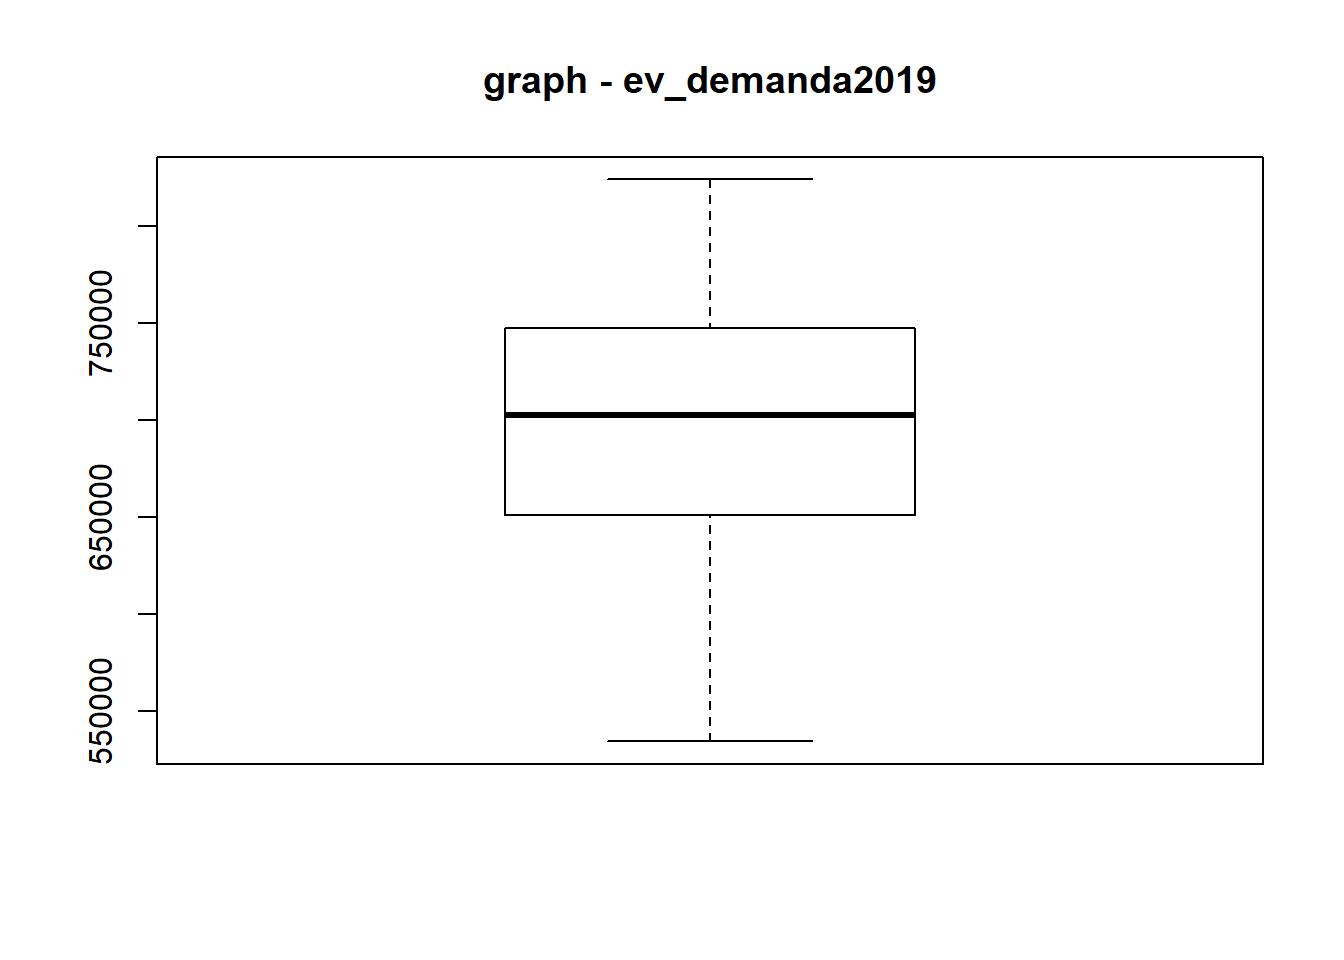
\includegraphics{Práctica-2_files/figure-latex/unnamed-chunk-15-1.pdf}

\textbf{Evolución demanda 2019-2020 (Abril)}

\begin{Shaded}
\begin{Highlighting}[]
\KeywordTok{plot}\NormalTok{(elect_apr}\OperatorTok{$}\NormalTok{day, elect_apr}\OperatorTok{$}\NormalTok{ev_demanda_}\DecValTok{2020}\NormalTok{, }\DataTypeTok{type=}\StringTok{"overplotted"}\NormalTok{,   }\DataTypeTok{pch=}\DecValTok{1}\NormalTok{, }\DataTypeTok{col=}\StringTok{"blue"}\NormalTok{, }\DataTypeTok{xlab=}\StringTok{"Days"}\NormalTok{,    }\DataTypeTok{ylab=}\StringTok{"ev-demanda"}\NormalTok{,   }\DataTypeTok{main=}\StringTok{"Ev-demanda (April)"}\NormalTok{, }\DataTypeTok{ylim=}\KeywordTok{c}\NormalTok{(}\KeywordTok{min}\NormalTok{(elect}\OperatorTok{$}\NormalTok{ev_demanda_}\DecValTok{2020}\NormalTok{), }\KeywordTok{max}\NormalTok{(elect}\OperatorTok{$}\NormalTok{ev_demanda2019)))}
\KeywordTok{lines}\NormalTok{(elect_apr}\OperatorTok{$}\NormalTok{day, elect_apr}\OperatorTok{$}\NormalTok{ev_demanda2019,}\DataTypeTok{type=}\StringTok{"overplotted"}\NormalTok{,}\DataTypeTok{pch=}\DecValTok{2}\NormalTok{,}\DataTypeTok{col=}\StringTok{"red"}\NormalTok{)}
\KeywordTok{legend}\NormalTok{(}\StringTok{"topright"}\NormalTok{,}\DataTypeTok{legend=}\KeywordTok{c}\NormalTok{(}\StringTok{"2020"}\NormalTok{,}\StringTok{"2019"}\NormalTok{),    }\DataTypeTok{pch=}\KeywordTok{c}\NormalTok{(}\DecValTok{1}\NormalTok{,}\DecValTok{2}\NormalTok{),}\DataTypeTok{col=}\KeywordTok{c}\NormalTok{(}\StringTok{"blue"}\NormalTok{,}\StringTok{"red"}\NormalTok{))}
\end{Highlighting}
\end{Shaded}

\includegraphics{Práctica-2_files/figure-latex/unnamed-chunk-16-1.pdf}

{ \emph{SERGIO, resultados presentados en práctica 1}}

\hypertarget{resoluciuxf3n-del-problema}{%
\section{6. Resolución del problema}\label{resoluciuxf3n-del-problema}}

{ \emph{SERGIO y Alejandro}}

\end{document}
